\section{Model Comparison Results}
\label{sec:5_2}

Four model variants were evaluated on the fixed temporal split (train: Dec 2024--Jun 2025, test: Jun--Jul 2025). Each model configuration was trained three times with different random seeds to assess variance. Results are reported as mean $\pm$ standard deviation across runs.

\begin{figure}[htbp]
    \centering
    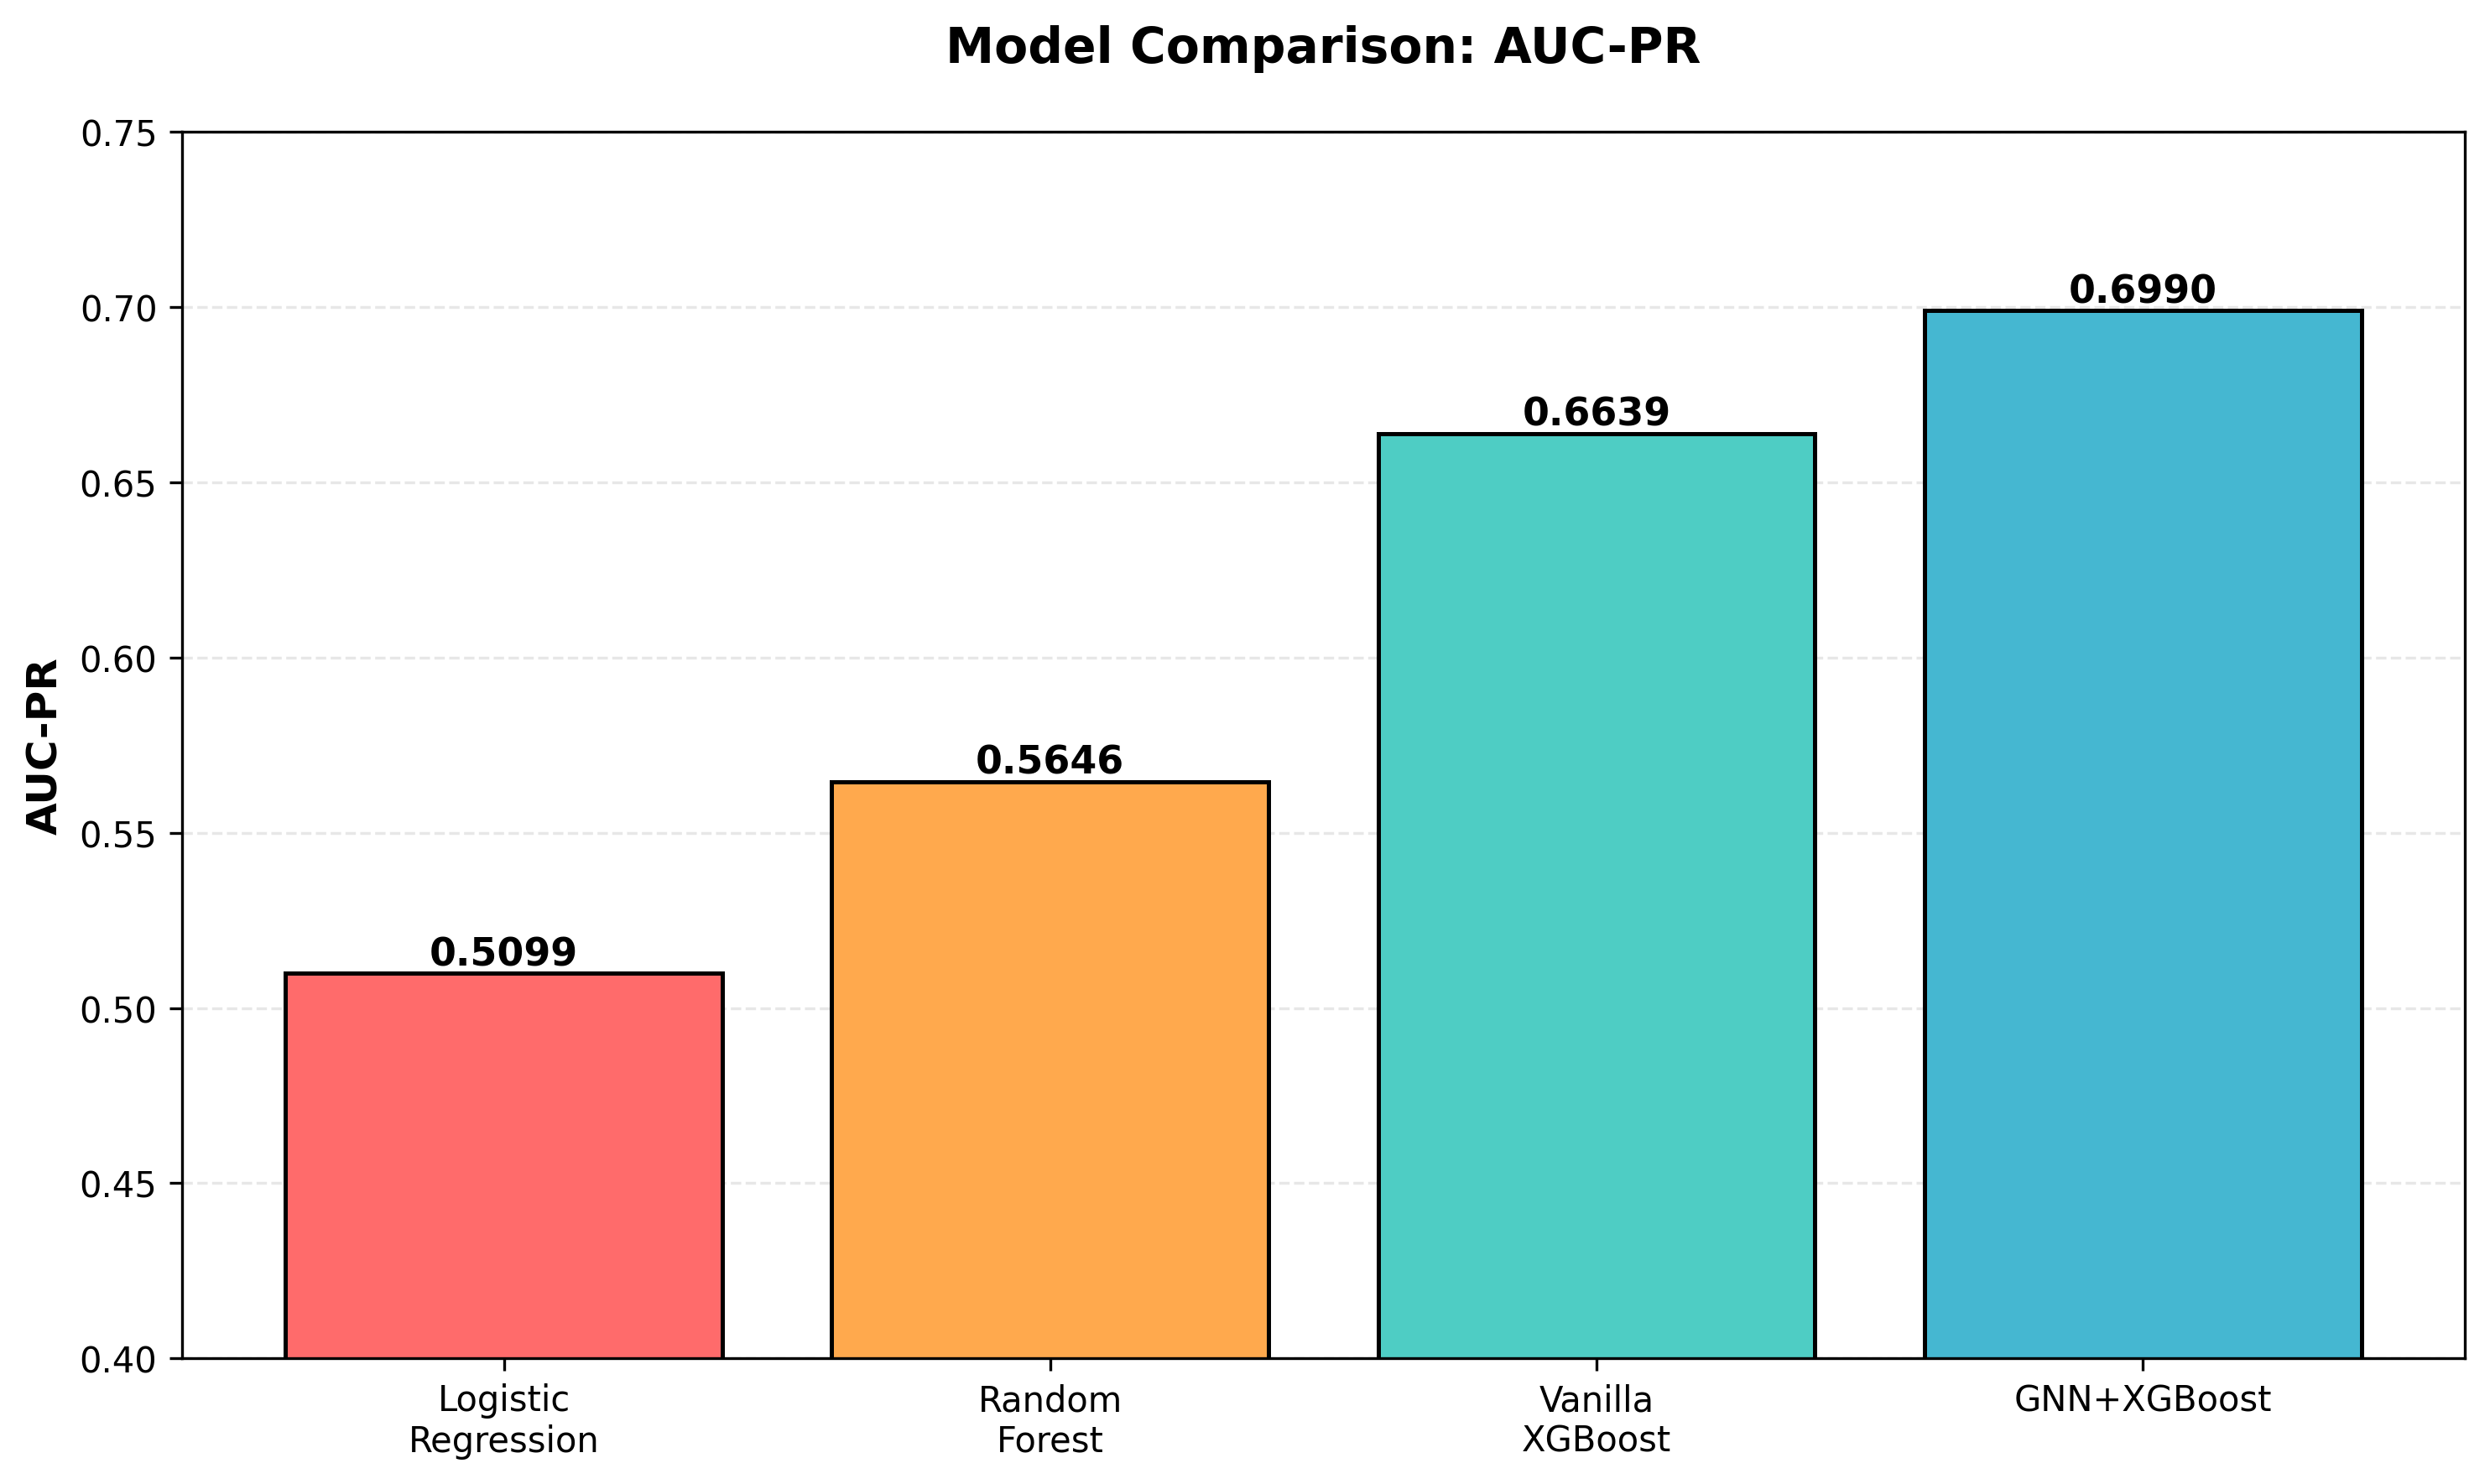
\includegraphics[width=0.8\textwidth]{figures/fig_5_5_2_1.png}
    \caption{Model Comparison: AUC-PR}
    \label{fig:5_3}
\end{figure}

\begin{table}[htbp]
    \centering
    \caption{Model Comparison with Variance (n=3 runs per model)}
    \label{tab:5_1}
    \begin{tabular}{lcccc}
        \toprule
        Model & AUC-PR & AUC-ROC & Precision & Recall \\
        \midrule
        Logistic Regression & 0.577 $\pm$ 0.117 & 0.946 $\pm$ 0.017 & 0.214 $\pm$ 0.125 & 0.872 $\pm$ 0.031 \\
        Random Forest & 0.621 $\pm$ 0.078 & 0.953 $\pm$ 0.008 & 0.488 $\pm$ 0.114 & 0.827 $\pm$ 0.039 \\
        Vanilla XGBoost & 0.733 $\pm$ 0.063 & 0.958 $\pm$ 0.003 & 0.746 $\pm$ 0.070 & 0.671 $\pm$ 0.042 \\
        GNN+XGBoost & 0.733 $\pm$ 0.058 & 0.950 $\pm$ 0.009 & 0.758 $\pm$ 0.053 & 0.673 $\pm$ 0.047 \\
        \bottomrule
    \end{tabular}
\end{table}

\textbf{Key Findings:}

Both XGBoost variants achieve comparable AUC-PR performance (0.733), substantially outperforming Random Forest (0.621) and Logistic Regression (0.577) baselines. The graph-augmented model shows minimal marginal improvement over tabular-only XGBoost (mean difference: +0.0006, 0.08\%), though with slightly higher precision (0.758 vs 0.746) at equivalent recall.

The relatively high standard deviations (0.063 for vanilla, 0.058 for GNN) indicate sensitivity to train/test split composition, with individual runs ranging from 0.664 to 0.789 AUC-PR. This variance reflects the challenge of fraud detection on imbalanced data (8.11\% fraud rate) and motivates the temporal cross-validation analysis in Section~\ref{sec:5_7}.

XGBoost's dominance over linear models confirms that non-linear feature interactions are critical for fraud detection. The SHAP analysis (Section~\ref{sec:5_9}) reveals that GNN embeddings contribute 17.3\% of total feature importance, providing supplementary relational signal that complements tabular features rather than replacing them.

\textbf{Cross-Validation Validation:} To assess robustness beyond the fixed split, we conducted 5-fold temporal cross-validation with 7-day gaps. Vanilla XGBoost achieves mean CV AUC-PR of 0.2777 $\pm$ 0.0287, representing 62\% degradation from fixed-split performance (0.7327). This substantial drop reflects: (1) fraud rate decrease over time (1.97\% early period $\to$ 0.63\% late period), (2) temporal distribution shifts as fraud tactics evolve, and (3) sensitivity of precision-recall metrics to class imbalance changes. The high standard deviation ($\sigma$=0.029, coefficient of variation=10.3\%) indicates performance varies significantly across temporal windows.

Critically, this degradation mirrors the expanding window findings (Section~\ref{sec:5_5}): both vanilla XGBoost and GNN+XGBoost suffer when evaluated on temporally distant test sets without retraining. This validates that fraud detection requires \emph{frequent model updates} to maintain performance, a key operational consideration (Section~\ref{sec:5_10_3}). The fixed-split results represent best-case performance under favorable conditions, while cross-validation provides conservative estimates under temporal distribution shift.

\textbf{Precision@K Results:}

\begin{table}[htbp]
    \centering
    \caption{Precision@K Comparison (mean across 3 runs)}
    \label{tab:5_2}
    \begin{tabular}{lccc}
        \toprule
        Model & P@50 & P@100 & P@200 \\
        \midrule
        Vanilla XGBoost & 99.3\% & 97.7\% & 87.0\% \\
        GNN+XGBoost & 96.7\% & 98.0\% & 88.0\% \\
        Random Forest & 85.3\% & 81.7\% & 80.0\% \\
        Logistic Regression & 90.7\% & 83.3\% & 83.5\% \\
        \bottomrule
    \end{tabular}
\end{table}

Both XGBoost variants maintain exceptional precision at high-confidence thresholds, with P@100 exceeding 97\%. The hybrid model's P@200 of 88\% means 176 of the top 200 flagged listings are genuine fraud, providing high-quality review queues for fraud analysts. The near-perfect P@50 performance (97-99\%) indicates both models achieve extremely high precision when scoring listings with maximal confidence, making them suitable for automated blocking at strict thresholds.
